\documentclass[a4paper, 12pt]{report}

%%%%%%%%%%%%
% Packages %
%%%%%%%%%%%%

\usepackage[english]{babel}
\usepackage[noheader]{packages/sleek}
\usepackage{packages/sleek-title}
\usepackage{packages/sleek-theorems}
\usepackage{packages/sleek-listings}
\usepackage{amsmath}
\usepackage[normalem]{ulem}
\useunder{\uline}{\ul}{}
\usepackage{comment}
\usepackage{hyperref}
\usepackage{listings}
\lstset{language=Python}
\lstset{frame=lines}
\lstset{basicstyle=\footnotesize}
\usepackage{multirow}
\setcounter{tocdepth}{3}
\setcounter{secnumdepth}{3}
\graphicspath{ {figures/} }
\usepackage{array}
\definecolor{mygreen}{rgb}{0,0.6,0}
\definecolor{mygray}{rgb}{0.5,0.5,0.5}
\definecolor{mymauve}{rgb}{0.58,0,0.82}
\definecolor{myorange}{rgb}{0.855,0.576,0.027}

%%%%%%%%%%%%%%
% Title-page %
%%%%%%%%%%%%%%

\logo{./resources/pdf/logo.pdf}
\institute{Department Of Aerospace Engineering}
\faculty{AS2101\\Prof. Bharath Govindarajan\\Prof. Ramakrishna M }
\title{ROOT FINDING ALGORITHMS\\TASK 3: 24-07-2021(Due-Date) }
\subtitle{REPORT}
\author{\textbf{AUTHOR}\\Yash Singh Jha-(AE19B016)\\ }

 \date{July 24 , 2021}


%%%%%%%%%%%%%%%%
% Bibliography %
%%%%%%%%%%%%%%%%

\addbibresource{./resources/bib/references.bib}

%%%%%%%%%%
% Others %
%%%%%%%%%%

\lstdefinestyle{latex}{
    language=TeX,
    style=default,
    %%%%%
    commentstyle=\ForestGreen,
    keywordstyle=\TrueBlue,
    stringstyle=\VeronicaPurple,
    emphstyle=\TrueBlue,
    %%%%%
    emph={LaTeX, usepackage, textit, textbf, textsc}
}

\FrameTBStyle{latex}

\def\tbs{\textbackslash}

%%%%%%%%%%%%
% Document %
%%%%%%%%%%%%

\begin{document}
    \maketitle
    \romantableofcontents
    \listoffigures
    \listoftables
    \begin{abstract}
    This document is like a summary report of the work we were assigned as Task 3 in the course As2101.\\
    This report presents a few of the various methods/algorithms used to calculate the root/zeros/ciphers of a function. We discuss three main methods - Bisection method , Newton's method and Secant method.\\
    Chapter 1 - Root-finding Algorithms, deals with the theory behind each of the three methods and illustrates it elegantly using appropriate equations and figures.\\
    Chapter 2 - Numerical Computation, presents and discusses the three methods in Python -  their characteristics and differences.\\
    Chapter 3 - Results, takes us through the results of the Python codes presented in chapter 2 and compares the computational differences between them.\\
    Chapter 4- Newton's Method : Additional Example, takes us through the special example, as asked to do.\\
    Chapter 5 - Conclusion, presents a concluding remark on the overall report and the materials covered.It also gives a comment on the relative execution speeds of the three method.\\
    This LaTeX file itself is the part of the task for the third week of AS2101.
    \end{abstract}
    
    \chapter{Root-Finding Algorithms}
In mathematics and computing, a root-finding algorithm is an algorithm for finding zeroes, also called "roots", of continuous functions. A zero of a function f, from the real numbers to real numbers or from the complex numbers to the complex numbers, is a number x such that f(x) = 0. As, generally, the zeroes of a function cannot be computed exactly nor expressed in closed form, root-finding algorithms provide approximations to zeroes, expressed either as floating point numbers or as small isolating intervals, or disks for complex roots (an interval or disk output being equivalent to an approximate output together with an error bound / tolerance).\\
Solving an equation $f(x) = g(x)$ is the same as finding the roots of the function $h(x) = f(x) – g(x)$. Thus root-finding algorithms allow solving any equation defined by continuous functions. However, most root-finding algorithms do not guarantee that they will find all the roots; in particular, if such an algorithm does not find any root, that does not mean that no root exists.\\
Most numerical root-finding methods use iteration, producing a sequence of numbers that hopefully converge towards the root as a limit. They require one or more initial guesses of the root as starting values, then each iteration of the algorithm produces a successively more accurate approximation to the root. Since the iteration must be stopped at some point these methods produce an approximation to the root, not an exact solution. Many methods compute subsequent values by evaluating an auxiliary function on the preceding values. The limit is thus a fixed point($f(c) = c$) of the auxiliary function, which is chosen for having the roots of the original equation as fixed points, and for converging rapidly to these fixed points.\\
The behaviour of general root-finding algorithms is studied in numerical analysis. However, for polynomials, root-finding study belongs generally to computer algebra, since algebraic properties of polynomials are fundamental for the most efficient algorithms. The efficiency of an algorithm may depend dramatically on the characteristics of the given functions. For example, many algorithms use the derivative of the input function, while others work on every continuous function. In general, numerical algorithms are not guaranteed to find all the roots of a function, so failing to find a root does not prove that there is no root. However, for polynomials, there are specific algorithms that use algebraic properties for certifying that no root is missed, and locating the roots in separate intervals (or disks for complex roots) that are small enough to ensure the convergence of numerical methods (typically Newton's method) to the unique root so located.
    \section{Bisection Method}
    In mathematics, the bisection method is a root-finding method that applies to any continuous functions for which one knows two values with opposite signs. The method consists of repeatedly bisecting the interval defined by these values and then selecting the sub-interval in which the function changes sign, and therefore must contain a root. It is a very simple and robust method, but it is also relatively slow. Because of this, it is often used to obtain a rough approximation to a solution which is then used as a starting point for more rapidly converging methods. The method is also called the interval halving method, the binary search method, or the dichotomy method.
    Figure~\ref{fig:BM}\\ shows a few steps of the bisection method.
    \begin{figure}[h]
    \centering
    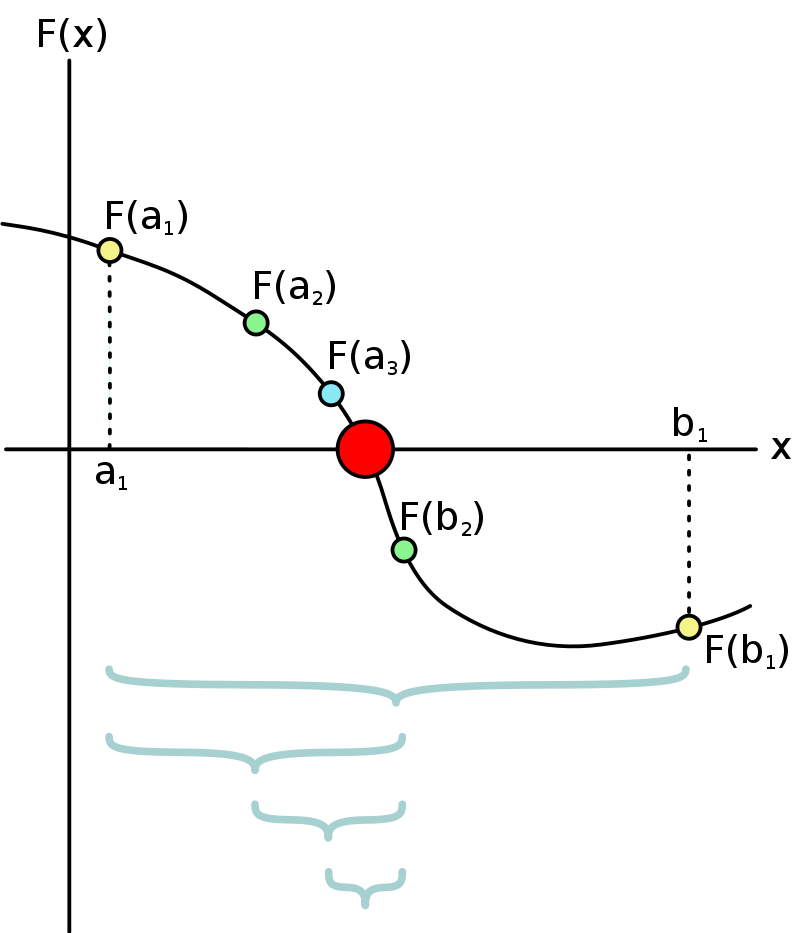
\includegraphics[width=10cm]{Bisection Method.png}
    \caption{A few steps of the bisection method applied over the starting range $[a_{1};b_{1}]$.}
    \label{fig:BM}
    \end{figure}
    \subsubsection{Method}
    The method is applicable for numerically solving the equation $f(x) = 0$ for the real variable x, where f is a continuous function defined on an interval $[a, b]$ and where $f(a)$ and $f(b)$ have opposite signs. In this case a and b are said to bracket a root since, by the intermediate value theorem, the continuous function f must have at least one root in the interval $(a,b)$.\\
    At each step the method divides the interval in two by computing the midpoint $c = (a+b) / 2$ of the interval and the value of the function $f(c)$ at that point. Unless c is itself a root (which is very unlikely, but possible) there are now only two possibilities: either $f(a)$ and $f(c)$ have opposite signs and bracket a root, or $f(c)$ and $f(b)$ have opposite signs and bracket a root. The method selects the sub-interval that is guaranteed to be a bracket as the new interval to be used in the next step. In this way an interval that contains a zero of f is reduced in width by 50\% at each step. The process is continued until the interval is sufficiently small.
    \subsubsection{Iteration Tasks}
    The input for the method is a continuous function f, an interval $[a, b]$, and the function values $f(a)$ and $f(b)$. The function values are of opposite sign (there is at least one zero crossing within the interval). Each iteration performs these steps:
    \begin{enumerate}
        \item Calculate c, the midpoint of the interval, $c = (a+b)/2$
        \item Calculate the function value at the midpoint, $f(c)$
        \item If convergence is satisfactory (that is, $c - a$ is sufficiently small, or $|f(c)|$ is sufficiently small), return c and stop iterating.
        \item Examine the sign of $f(c)$ and replace either $(a, f(a))$ or $(b, f(b))$ with $(c, f(c))$ so that there is a zero crossing within the new interval.
    \end{enumerate}
    When implementing the method on a computer, there can be problems with finite precision, so there are often additional convergence tests or limits to the number of iterations. Although f is continuous, finite precision may preclude a function value ever being zero. For example, consider $f(x)$ = x − $\pi$; there will never be a finite representation of x that gives zero. Additionally, the difference between a and b is limited by the floating point precision; i.e., as the difference between a and b decreases, at some point the midpoint of $[a, b]$ will be numerically identical to (within floating point precision of) either a or b.
    \subsubsection{Example: Finding the root of a polynomial}
    Suppose that the bisection method is used to find a root of the polynomial :
    \begin{equation}
      f(x) = x^{3} - x - 2  
    \end{equation}
    First, two numbers a and b have to be found such that $f(a)$ and $f(b)$ have opposite signs. For the above function, $a=1$ and $b=2$ satisfy the criterion, as:
    \begin{equation}
      f(1) = (1)^{3} - (1) - 2  = -2
    \end{equation}
    and 
    \begin{equation}
      f(2) = (2)^{3} - (2) - 2  = +4
    \end{equation}
    Because the function is continuous, there must be a root within the interval $[1, 2]$.\\
    In the first iteration, the end points of the interval which brackets the root are $a_{1} = 1$ and $b_{1} = 2$, so the midpoint is:
    \begin{equation}
      c_{1} = \frac{2+1}{2} = 1.5
    \end{equation}
    The function value at the midpoint is $f(c_{1}) = (1.5)^{3} - (1.5) - 2 = -0.125$.Because $f(c_{1})$ is negative, a=1 is replaced with a = 1.5 for the next iteration to ensure that $f(a)$ and $f(b)$ have opposite signs. As this continues, the interval between a and b will become increasingly smaller, converging on the root of the function. See this happen in the table below: (The following values were obtained using the code (\ref{lst:BM}) with the tolerance value of 0.0001).
    \begin{table}[]
\begin{tabular}{|c|l|l|l|l|}
\hline
\textbf{iter} & \multicolumn{1}{c|}{\textbf{a}} & \multicolumn{1}{c|}{\textbf{b}} & \multicolumn{1}{c|}{\textbf{c}} & \multicolumn{1}{c|}{\textbf{f(c)}} \\ \hline
\textbf{1}  & 1.000000000000 & 2.000000000000 & 1.500000000000 & -0.125000000000 \\ \hline
\textbf{2}  & 1.500000000000 & 2.000000000000 & 1.750000000000 & 1.609375000000  \\ \hline
\textbf{3}  & 1.500000000000 & 2.000000000000 & 1.625000000000 & 0.666015625000  \\ \hline
\textbf{4}  & 1.500000000000 & 1.750000000000 & 1.562500000000 & 0.252197265625  \\ \hline
\textbf{5}  & 1.500000000000 & 1.625000000000 & 1.531250000000 & 0.059112548828  \\ \hline
\textbf{6}  & 1.500000000000 & 1.562500000000 & 1.515625000000 & -0.034053802490 \\ \hline
\textbf{7}  & 1.515625000000 & 1.531250000000 & 1.523437500000 & 0.012250423431  \\ \hline
\textbf{8}  & 1.515625000000 & 1.523437500000 & 1.519531250000 & -0.010971248150 \\ \hline
\textbf{9}  & 1.519531250000 & 1.523437500000 & 1.521484375000 & 0.000622175634  \\ \hline
\textbf{10} & 1.519531250000 & 1.521484375000 & 1.520507812500 & -0.005178886466 \\ \hline
\textbf{11} & 1.520507812500 & 1.521484375000 & 1.520996093750 & -0.002279443317 \\ \hline
\textbf{12} & 1.520996093750 & 1.521484375000 & 1.521240234375 & -0.000828905861 \\ \hline
\textbf{13} & 1.521240234375 & 1.521484375000 & 1.521362304688 & -0.000103433124 \\ \hline
\textbf{14} & 1.521362304688 & 1.521484375000 & 1.521423339844 & 0.000259354252  \\ \hline
\textbf{15} & 1.521362304688 & 1.521423339844 & 1.521392822266 & 0.000077956314  \\ \hline
\end{tabular}
\caption{Iteration Step Values for the Example illustrated for Bisection Method.}
\label{table:ISV}
\end{table}
    \section{Newton's Method}
    In numerical analysis, Newton's method, also known as the Newton–Raphson method, named after Isaac Newton and Joseph Raphson, is a root-finding algorithm which produces successively better approximations to the roots (or zeroes) of a real-valued function. The most basic version starts with a single-variable function f defined for a real variable x, the function's derivative $f'$, and an initial guess $x_{0}$ for a root of f. If the function satisfies sufficient assumptions and the initial guess is close, then:
    \begin{equation}
      x_{1} = x_{0} - \frac{f(x_{0})}{f'(x_{0})}
    \end{equation}
    is a better approximation of the root than $x_{0}$. Geometrically, $(x_{1},0)$ is the intersection of the x-axis and the tangent of the graph of f at $(x_{0},f(x_{0})$: that is, the improved guess is the unique root of the linear approximations at the initial point. The process is repeated as :
    \begin{equation}
        x_{n+1} = x_{n} - \frac{f(x_{n}}{f'(x_{n})}
    \end{equation}
    until a sufficiently precise value is reached. This algorithm is first in the class of Householder's methods, succeeded by Halley's method. The method can also be extended to complex functions and to systems of equations.
    \subsubsection{Method}
    The idea is to start with an initial guess which is reasonably close to the true root, then to approximate the function by its tangent line using calculus, and finally to compute the x-intercept of this tangent line by elementary algebra. This x-intercept will typically be a better approximation to the original function's root than the first guess, and the method can be iterated.\\
    Figure~\ref{fig:NM} shows s few steps of the Newton's Method.
    \begin{figure}[h]
    \centering
    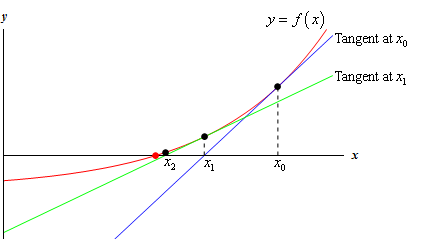
\includegraphics[width=10cm]{Newton's Method.png}
    \caption{A few iterations of the Newton's method.}
    \label{fig:NM}
    \end{figure}
    \subsubsection{Iteration Tasks}
    Suppose we need to solve the equation $f(x) = 0$ and $x=c$ is the actual root of $f(x)$. We assume that the function $f(x)$ is differentiable in an open interval that contains c.
    To find an approximate value for c:
    \begin{enumerate}
        \item Start with an initial approximation $x_{0}$ close to c.
        \item Determine the next approximation by the formula:
        \begin{equation}
        x_{1} = x_{0} - \frac{f(x_{0})}{f'(x_{0})}
        \end{equation}
        \item Continue the iterative process using the formula:
        \begin{equation}
        x_{n+1} = x_{n} - \frac{f(x_{n}}{f'(x_{n})}
        \end{equation}
    \end{enumerate}
    until the root is found to the desired accuracy.
    \subsubsection{Example: Finding the root of a polynomial }
    Consider the function(figure~\ref{fig:NMI}):
    \begin{equation}
        f(x) = x^{3} - 3x -3
    \end{equation}
    \begin{figure}[h]
    \centering
    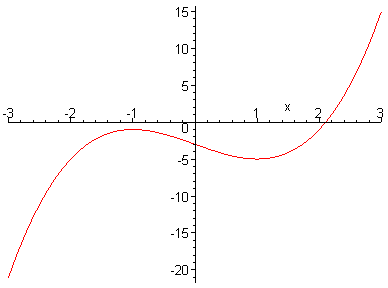
\includegraphics[width=10cm]{Newton's Method Image.png}
    \caption{Graph of the function used to illustrate Newton's Method.}
    \label{fig:NMI}
    \end{figure}
    We begin at a point $x_{0}=2$ and then we can find:
    \begin{equation}
        f(2) = (2)^{3} - 3(2)-3 = -1
    \end{equation}
    We also find 
    \begin{equation}
        f(2) = (2)^{3} - 3(2)-3 = -1
    \end{equation}
    The first Newton iterate is therefore
    \begin{equation}
        x_{1}= 2-\frac{-1}{9} = 2.111
    \end{equation}
    Now we find
    \begin{equation}
        f(19/9) = (\frac{19}{9})^{3} - 3\frac{19}{9} - 3 = .07545
    \end{equation}
    We also find
    \begin{equation}
        f'(19/9) = 3(\frac{19}{9})^{2} - 3 = 10.3704
    \end{equation}
    The second Newton iterate is therefore
    \begin{equation}
       x_{2} = 2.111-\frac{0.07545}{10.3704} = 2.1038
    \end{equation}
    And we continue similarly.
    
    \section{Secant Method}
    In numerical analysis, the secant method is a root-finding algorithm that uses a succession of roots of secant lines to better approximate a root of a function f. The secant method can be thought of as a finite-difference approximation of Newton's method. However, the secant method predates Newton's method by over 3000 years.
    \begin{figure}[h]
    \centering
    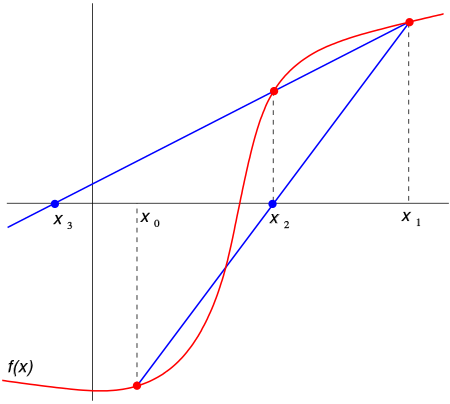
\includegraphics[width=10cm]{Secant Method.png}
    \caption{The first two iterations of the secant method..}
    \label{fig:SM}
    \end{figure}
    
    \subsubsection{Method and Iteration Tasks}
    The secant method is defined by the recurrence relation:
    \begin{equation}
       x_{n} = x_{n-1} - f(x_{n-1}) \frac{x_{n-1}-x_{n-2}}{f(x_{n-1})-f(x_{n-2})} = \frac{x_{n-2}f(x_{n-1}) - x_{n-1}f(x_{n-2})}{f(x_{n-1})-f(x_{n-2})}
    \end{equation}
    As can be seen from the recurrence relation, the secant method requires two initial values, $x_{0}$ and $x_{1}$, which should ideally be chosen to lie close to the root.
    
    We construct a line through the points $(x_{0}, f(x_{0}))$ and $(x_{1}, f(x_{1}))$, as shown in the picture above. In slope–intercept form, the equation of this line is
    \begin{equation}
        y = \frac{f(x_{1})-f(x_{0})}{x_{1}-x_{0}} (x-x_{1}) + f(x_{1})
    \end{equation}
    The root of this linear function, that is the value of x such that $y=0$ is:
    \begin{equation}
    x = x_{1} - f(x_{1})\frac{x_{1} - x_{0}}{f(x_{1}) -f(x_{0}) }
    \end{equation}
    We then use this new value of x as $x_{2}$ and repeat the process, using $x_{1}$ and $x_{2}$ instead of $x_{0}$ and $x_{1}$. We continue this process, solving for $x_{3}$,$x_{4}$ etc.,until we reach a sufficiently high level of precision (a sufficiently small difference between $x_{n}$ and $x_{n-1}$).:
    \begin{equation}
    x_{2} = x_{1} - f(x_{1})\frac{x_{1} - x_{0}}{f(x_{1}) -f(x_{0}) }
    \end{equation}
    \begin{equation}
    x_{3} = x_{2} - f(x_{2})\frac{x_{2} - x_{1}}{f(x_{2}) -f(x_{1}) }
    \end{equation}
    and so on till:
    \begin{equation}
    x_{n}= x_{n-1} - f(x_{n-1})\frac{x_{n-1} - x_{n-2}}{f(x_{n-1}) -f(x_{n-2}) }
    \end{equation}
    \subsubsection{Example: Finding the root of a polynomial}
    Consider the polynomial:
    \begin{equation}
        f(x) = x^{3} - x - 1
    \end{equation}
    First, we need to find the points $x_{0}$ and $x_{1}$ such that $x_{0}$< $x_{1}$ and $f(x_{0})$.$f(x_{0})$ <0. We take $x_{0}=1$ and $x_{1}=2$. So, $f(x_{0})=f(1)=-1$ and $f(x_{1})=f(2)=5$.\\
    \textbf{$1^{st}$ iteration:} $x_{0}=1$ and $x_{1}=2$.
    \begin{equation}
    x_{2} = x_{0} - f(x_{0})\frac{x_{1} - x_{0}}{f(x_{1}) -f(x_{0}) } = 1-(-1)\frac{2-1}{5-(-1)} = 1.6667
    \end{equation}
    \begin{equation}
        f(x_{2}) =f(1.6667) = -0.5787
    \end{equation}
    
    \textbf{$2^{nd}$ iteration:} $x_{1}=2$ and $x_{2}=1.6667$. So, $f(x_{1})=f(2)=5$ and $f(x_{2})=f(1.6667)=-0.5787$
    \begin{equation}
    x_{3} = x_{1} - f(x_{1})\frac{x_{2} - x_{1}}{f(x_{2}) -f(x_{1}) } = 2-(5)\frac{1.6667-2}{-0.5787-(5)} = 1.25311
    \end{equation}
    \begin{equation}
        f(x_{3}) =f(1.25311) = -0.28536
    \end{equation}
    and so on.


 \chapter{ Numerical Computation : Python Implementation}
This chapter takes us through the codes in Python used to implement the theory provided to us in the preceding chapter or in other words - here, we go through the Python Code for the numerical implementation of the Bisection Method, Newton's Method and the Secant Method.
\section{Bisection Method}
The following code in Python, is the implementation of the theory and iteration tasks covered in the previous chapters. The code is commented well so further explanation of the code doesn't seem necessary.Results of the code~\ref{lst:BM} are presented in the next chapter, in tables~\ref{table:1}, \ref{table:2}, \ref{table:3}and \ref{table:4} , correspondingly the plot ~\ref{fig:Plot1}.
\lstset{caption={Function named \textbf{'bisection'} is constructed to generate the iteration steps of the Bisection Method}}
\lstset{label={lst:BM}}
\begin{lstlisting}
def bisection(f,a,b,TOL,NMAX):
    # THIS FUNCTION PRINTS THE a,b,c VALUES FOR EACH ITERATION:
    
    #Approximates root using Bisection Method
    #In an interval[a,b] with a tolerance TOL
    #|f(c)| < TOL, where m is the midpoint
    

    #INPUT : f , a , b , TOL , NMAX
    # f : function / polynomial
    # a : interval start
    # b : interval end
    # TOL : tolerance value
    # NMAX : maximum number of iterations


    #Print Table Header:
    print('----------------------------------------------------------------')
    print('iter \t\t a \t\t b \t\t c \t\t f(c)        ')
    print('------------------------------------------------------------------')
    #satisfy the conditions needed to apply the Bisection Method:
    if np.sign(f(a)) == np.sign(f(b)):
        print("No root found in the given interval!")
        exit()
        
    for i in range(NMAX):
        #Compute Midpoint
        c = (a+b)/2
        #print line for the table:
        N.append(1+i)
        f_x.append(f(c))
        print(str(1+i)+'\t% 15.12f\t% 15.12f\t% 15.12f\t% 15.12f\t' %(a, b, c, f(c)))
        #Check stopping condition:
        if np.abs(f(c)) < TOL:
            print('------------------------------------------------------------')
            print('Root Found: '+str(c))
            break
        #Implement Recursion:
        elif np.sign(f(a)) == np.sign(f(c)):
            #Improvement on a
            a = c
        elif np.sign(f(b)) == np.sign(f(c)):
            #Improvement on b
            b = c
        
    if i == NMAX -1:
        print("MAX NUMBER OF ITERATIONS REACHED!")
        print('Approximaiton to the Root after max iterations is : '+str(c))        
        exit()
\end{lstlisting}
\section{Newton's Method}
The task is repeated for Newton's method here. For reference and better inference of the code, parallel viewing of the codes(\ref{lst:NM}) and the results(tables~\ref{table:5}, \ref{table:6}, \ref{table:7}and \ref{table:8} , correspondingly plot ~\ref{fig:Plot2}) provided in the next chapter is advised.
\lstset{caption={Function named \textbf{'newton'} is constructed to generate the iteration steps of the Newton's Method}}
\lstset{label={lst:NM}}
\begin{lstlisting}
def newton(f,fp,x0,TOL,NMAX):
    #INPUT : f , fp , x0 , TOL , NMAX
    # f : function / polynomial
    # fp : derivative of f
    # x0 : initial guess
    # TOL : tolerance value
    # NMAX : maximum number of iterations

    #Approximates root using Newton's Method
    #Recursive Program
    # Print Header
    print('--------------------------------------------------------------------------')
    print('iter \t\t xi \t\t   correction \t\t   rdiff        ')
    print('--------------------------------------------------------------------------')
    # initiate values for  iteration loop:
    rdiff = 1
    xi = x0
    counter = 0
    while rdiff > TOL and counter < NMAX:
        # get the number of necessary iterations at that particular x0
        # compute relative difference
        rdiff = np.abs(f(xi)/fp(xi)/xi)
        # next xi:
        x1 = xi - f(xi)/fp(xi)
        N.append(counter+1)
        f_x.append(f(x1))
        # print iteration data:
        print('%i \t %15.12f \t %15.12f \t %15.12f' % (counter+1, x1, np.abs(f(xi)/fp(xi)),  rdiff))
        # prepare for the next iteration:
        xi = x1
        counter += 1
        if counter == NMAX:
            print("MAX NUMBER OF ITERATIONS REACHED!")
            print('Approximaiton to the Root after max iterations is : ' , x1)        
            exit()
    
    print('------------------------------------------------------------------------')
    print('Root Found: ', x1)
\end{lstlisting}    
\section{Secant Method}
The same process is repeated for the Secant Method. Codes(\ref{lst:SM}) and results (tables~\ref{table:9}, \ref{table:10}, \ref{table:11}and \ref{table:12} , correspondingly plot ~\ref{fig:Plot3}) are recommended to be observed in parallel.
\lstset{caption={Function named \textbf{'secant'} is constructed to generate the iteration steps of the Secant Method}}
\lstset{label={lst:SM}}
\begin{lstlisting}
def secant(f,x0,x1,TOL,NMAX):
    #INPUT : f , x0 , x1 , TOL , NMAX
    # f : function / polynomial
    # x0 : first initial point/guess
    # x1 : second initial point/guess
    # TOL : tolerance value
    # NMAX : maximum number of iterations

    #Approximates root using Secant Method

    #Print Header
    print('--------------------------------------------------------------------------')
    print("iter \t\t\t x2 \t\t\t\t f(x2)")
    print('--------------------------------------------------------------------------')
    
    for i in range(NMAX):
        if f(x0) == f(x1):
            print('DIVIDE BY ZERO ENCOUNTERED!')
            exit()
        #improved guess
        x2 = x0 - (x1-x0)*f(x0)/(f(x1)-f(x0))
        N.append(1+i)
        f_x.append(f(x2))
        #print values after each iteration step
        print("%d \t\t %15.12f \t\t %15.12f" %(1+i,x2,f(x2)))
        x0 = x1
        x1 = x2

        #executing the required precision
        if abs(f(x2)) < TOL:
            print('--------------------------------------------------------------------------')
            print('Root Found : ',x2)
            break
    #limiting number of iterations
    if i == NMAX -1:
        print("MAX NUMBER OF ITERATIONS REACHED!")
        print('Approximaiton to the Root after max iterations is : '+str(c))        
        exit()
\end{lstlisting}

\section{Tic-Toc Generator}
We have defined functions such that they enable us to measure the time required for the execution for various root finding algorithms.Listing ~\ref{lst:tictoc} contains the code for the generator. To understand the usage of the functions, please refer the next chapter for the results.
\lstset{caption={\textbf{tic() and toc()}}}
\lstset{label={lst:tictoc}}
\begin{lstlisting}
import time
def TicTocGenerator():
  # Function that returns time differences
  ti = 0           # initial time
  tf = time.time() # final time
  while True:
    ti = tf
    tf = time.time()
    yield (tf-ti)   #Returns the time difference

TicToc = TicTocGenerator()  #create an instance of the TicTocGenerator

# Main function through which we define both tic() and toc()
def toc(tempBool = True):
  # Prints the time difference yielded by instance of TicTocGenerator()-TicToc
  tempTimeInterval = next(TicToc)
  if tempBool:
    print("Elapsed time: %f seconds.\n" %tempTimeInterval)

def tic():
  # Records a time in TicToc, marks the beginning of a time interval
  toc(False)
\end{lstlisting}
\section{Task}
Consider the following functions:
\begin{equation}
    f_{1}(x) = x^{3} - 3 x^{2} - x + 9
\end{equation}
and,
\begin{equation}
    f_{2}(x) = \exp^{x}(x^{3} - 3 x^{2} - x + 9)
\end{equation}
\begin{figure}[h]
    \centering
    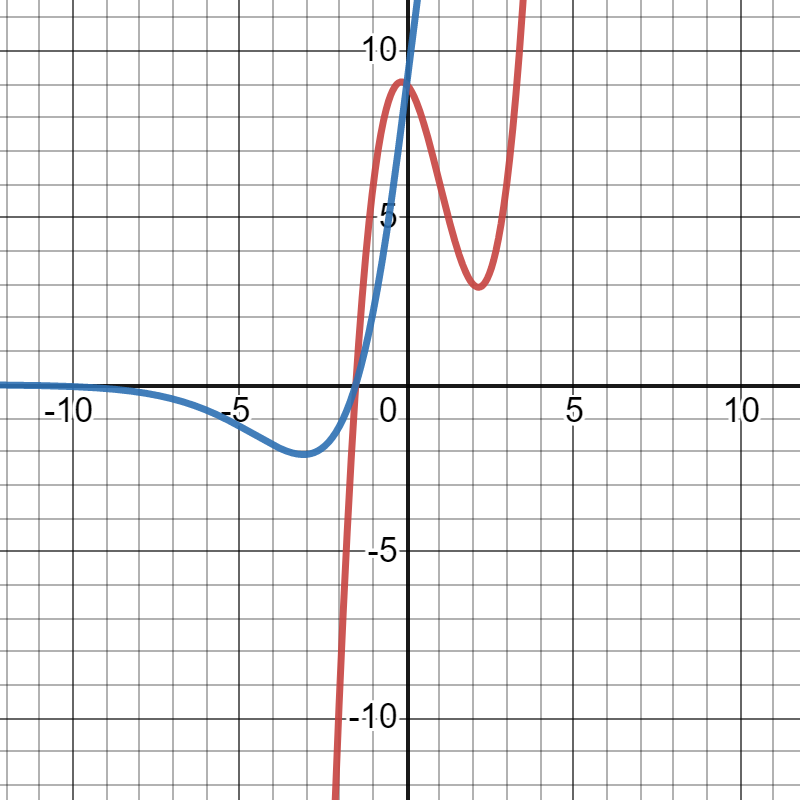
\includegraphics[width=10cm]{Funcs.png}
    \caption{Functions used to produce results ::Red : $f_{1}(x)$ ; Blue : $f_{2}(x)$.}
    \label{fig:Funcs}
    \end{figure}
    
The above functions look as shown in figure~\ref{fig:Funcs}. The root of the functions is -1.525.\\
Following points are important from the perspective of the results presented in the next chapter.
\begin{enumerate}
    \item The tolerance value (TOL) is kept a constant ($10^{10}$) through out.
    \item The maximum number of iterations(NMAX) is maintained at 1000, which is large enough to consider NMAX unimportant.
    \item Since, the root value is equal to -1.525, it was logical to have our initial intervals as $[a_{1},b_{1}] = [-5,0]$ and $[a_{2},b_{2}] = [-2.5,1]$ for the \textbf{Bisection Method}.
    \item Similarly, as initial guesses, $x_{0}^{1} = -2$ and $x_{0}^{2} = 5$ were chosen for the \textbf{Newton's Method}.
    \item Following the trend, as initial guesses $[x_{0},x_{1}] = [-2,5]$ and $[-2.5,1.5]$ were taken, for the \textbf{Secant Method}.
\end{enumerate}
\chapter{Results}
This chapter takes us through the results obtained by executing the various root finding algorithms. Results include the plots for $f(x)$ vs N, the values at the end of every iteration step and comparison of the execution time for each root finding algorithm.\\
Note: The execution times stated here are majorly dependent on the way I have implemented the maths into the python code. However, it gives a brief sense of the relative efficiencies of the methods.
\section{Plots}
Here, we present the plots obtained from the root finding algorithms.Figure~\ref{fig:Plot1}, \ref{fig:Plot2} and \ref{fig:Plot3} are the plots for the root finding algorithms, implemented for $f_{1}(x)$ and $f_{2}(x)$ with a tolerance value (TOL) and NMAX as specified earlier.\\
Tables~\ref{table:1}, \ref{table:2}, \ref{table:3}and \ref{table:4} correspond to the plots in \ref{fig:Plot1}.Tables~\ref{table:5}, \ref{table:6}, \ref{table:7}and \ref{table:8} correspond to the plots in \ref{fig:Plot2}. Tables~\ref{table:9}, \ref{table:10}, \ref{table:11}and \ref{table:12} correspond to the plots in \ref{fig:Plot3}.

\begin{figure}[!h]
\centering
\begin{subfigure}{.55\textwidth}
  \centering
  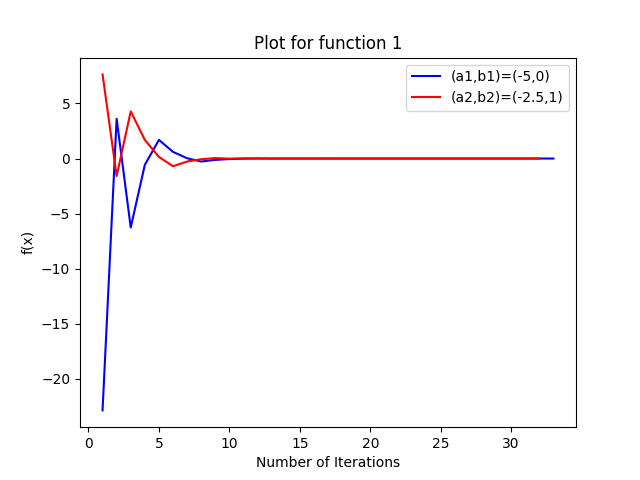
\includegraphics[width=.95\linewidth]{BM1.png}
  \caption{Plots for $f_{1}(x) vs N$.}
\end{subfigure}%
\begin{subfigure}{.55\textwidth}
  \centering
  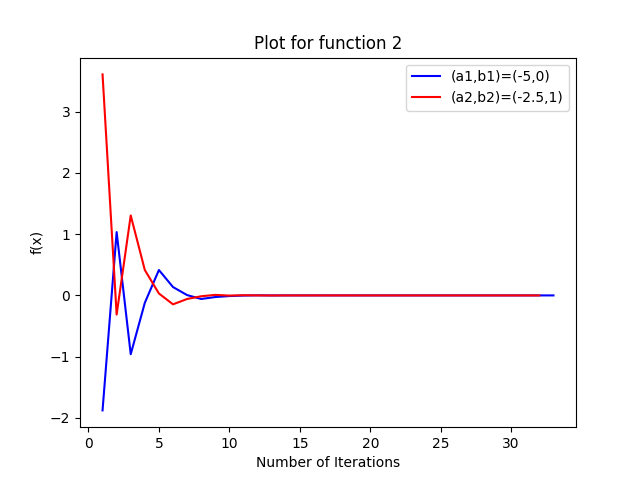
\includegraphics[width=.95\linewidth]{BM2.png}
  \caption{Plots for $f_{2}(x) vs N$.}
\end{subfigure}
\caption{Plots for \textbf{Bisection Method}.}
\label{fig:Plot1}
\end{figure}

\begin{figure}[!h]
\centering
\begin{subfigure}{.55\textwidth}
  \centering
  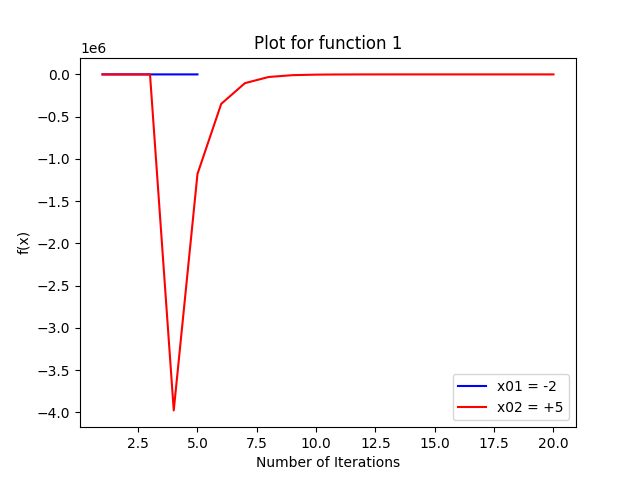
\includegraphics[width=.95\linewidth]{NM1.png}
  \caption{Plots for $f_{1}(x) vs N$.}
\end{subfigure}%
\begin{subfigure}{.55\textwidth}
  \centering
  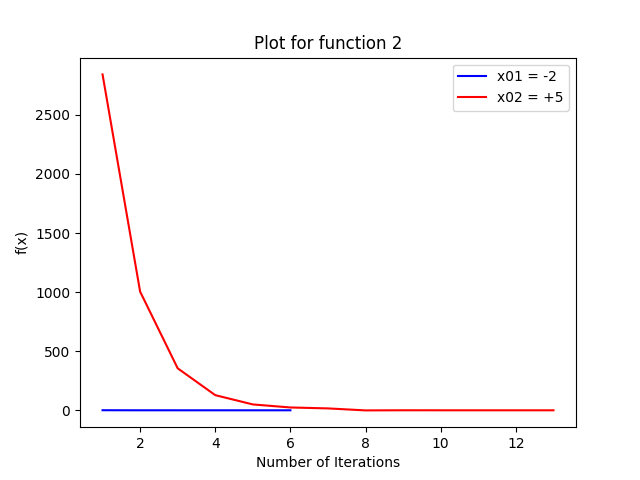
\includegraphics[width=.95\linewidth]{NM2.png}
  \caption{Plots for $f_{2}(x) vs N$.}
\end{subfigure}
\caption{Plots for \textbf{Newton's Method}.}
\label{fig:Plot2}
\end{figure}

\begin{figure}[h]
\centering
\begin{subfigure}{.55\textwidth}
  \centering
  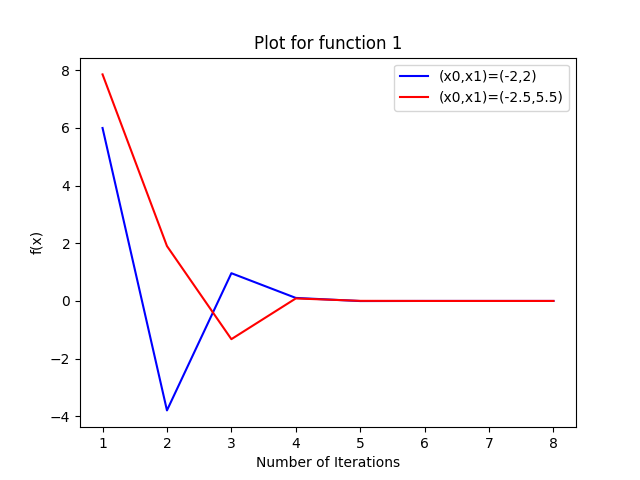
\includegraphics[width=.95\linewidth]{SM1.png}
  \caption{Plots for $f_{1}(x) vs N$.}
\end{subfigure}%
\begin{subfigure}{.55\textwidth}
  \centering
  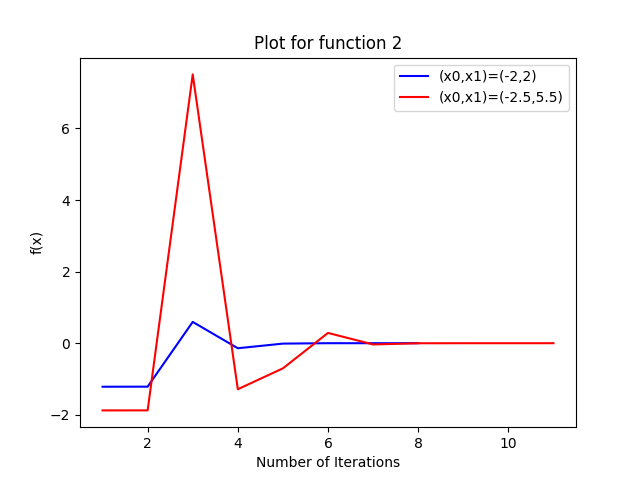
\includegraphics[width=.95\linewidth]{SM2.png}
  \caption{Plots for $f_{2}(x) vs N$.}
\end{subfigure}
\caption{Plots for \textbf{Secant Method}.}
\label{fig:Plot3}
\end{figure}


\section{Iteration Values}
This section contains the iteration values for Bisection Method applied for both the functions.\\
\begin{table}[!h]
\begin{tabular}{|l|l|l|l|l|}
\hline
\multicolumn{1}{|c|}{\textbf{iter}} &
  \multicolumn{1}{c|}{\textbf{a}} &
  \multicolumn{1}{c|}{\textbf{b}} &
  \multicolumn{1}{c|}{\textbf{c}} &
  \multicolumn{1}{c|}{\textbf{f(c)}} \\ \hline
\multicolumn{1}{|c|}{\textbf{1}}  & -5.000000000000 & 0.000000000000  & -2.500000000000 & -0.125000000000 \\ \hline
\multicolumn{1}{|c|}{\textbf{2}}  & -2.500000000000 & 0.000000000000  & -1.250000000000 & 1.609375000000  \\ \hline
\multicolumn{1}{|c|}{\textbf{3}}  & -2.500000000000 & -1.250000000000 & -1.875000000000 & 0.666015625000  \\ \hline
\multicolumn{1}{|c|}{\textbf{4}}  & -1.875000000000 & -1.250000000000 & 1.562500000000  & 0.252197265625  \\ \hline
\multicolumn{1}{|c|}{\textbf{5}}  & 1.562500000000  & -1.250000000000 & -1.406250000000 & 0.059112548828  \\ \hline
\multicolumn{1}{|c|}{\textbf{6}}  & 1.562500000000  & -1.406250000000 & -1.484375000000 & -0.034053802490 \\ \hline
\multicolumn{1}{|c|}{\textbf{7}}  & 1.562500000000  & -1.484375000000 & -1.523437500000 & 0.012250423431  \\ \hline
\multicolumn{1}{|c|}{\textbf{8}}  & 1.562500000000  & -1.523437500000 & -1.542968750000 & -0.010971248150 \\ \hline
\multicolumn{1}{|c|}{\textbf{9}}  & -1.542968750000 & -1.523437500000 & -1.533203125000 & 0.000622175634  \\ \hline
\multicolumn{1}{|c|}{\textbf{10}} & -1.533203125000 & -1.523437500000 & -1.528320312500 & -0.005178886466 \\ \hline
\multicolumn{1}{|c|}{\textbf{11}} & -1.528320312500 & -1.523437500000 & -1.525878906250 & -0.002279443317 \\ \hline
\multicolumn{1}{|c|}{\textbf{12}} & -1.525878906250 & -1.523437500000 & -1.524658203125 & -0.000828905861 \\ \hline
\multicolumn{1}{|c|}{\textbf{13}} & -1.525878906250 & -1.524658203125 & -1.525268554688 & -0.000103433124 \\ \hline
\multicolumn{1}{|c|}{\textbf{14}} & -1.525268554688 & -1.524658203125 & -1.524963378906 & 0.000259354252  \\ \hline
\multicolumn{1}{|c|}{\textbf{15}} & -1.525268554688 & -1.524963378906 & -1.525115966797 & 0.000077956314  \\ \hline
\textbf{16}                       & -1.525115966797 & -1.524963378906 & -1.525039672852 & 0.000946736811  \\ \hline
\textbf{17}                       & -1.525115966797 & -1.525039672852 & -1.525077819824 & 0.000369658372  \\ \hline
\textbf{18}                       & -1.525115966797 & -1.525077819824 & -1.525096893311 & 0.000081110886  \\ \hline
\textbf{19}                       & -1.525115966797 & -1.525096893311 & -1.525106430054 & -0.000063164925 \\ \hline
\textbf{20}                       & -1.525106430054 & -1.525096893311 & -1.525101661682 & 0.000008973153  \\ \hline
\textbf{21}                       & -1.525106430054 & -1.525101661682 & -1.525104045868 & -0.000027095843 \\ \hline
\textbf{22}                       & -1.525104045868 & -1.525101661682 & -1.525102853775 & -0.000009061334 \\ \hline
\textbf{23}                       & -1.525102853775 & -1.525101661682 & -1.525102257729 & -0.000000044088 \\ \hline
\textbf{24}                       & -1.525102257729 & -1.525101661682 & -1.525101959705 & 0.000004464533  \\ \hline
\textbf{25}                       & -1.525102257729 & -1.525101959705 & -1.525102108717 & 0.000002210223  \\ \hline
\textbf{26}                       & -1.525102257729 & -1.525102108717 & -1.525102183223 & 0.000001083067  \\ \hline
\textbf{27}                       & -1.525102257729 & -1.525102183223 & -1.525102220476 & 0.000000519490  \\ \hline
\textbf{28}                       & -1.525102257729 & -1.525102220476 & -1.525102239102 & 0.000000237701  \\ \hline
\textbf{29}                       & -1.525102257729 & -1.525102239102 & -1.525102248415 & 0.000000096806  \\ \hline
\textbf{30}                       & -1.525102257729 & -1.525102248415 & -1.525102253072 & 0.000000026359  \\ \hline
\textbf{31}                       & -1.525102257729 & -1.525102253072 & -1.525102255400 & -0.000000008864 \\ \hline
\textbf{32}                       & -1.525102255400 & -1.525102253072 & -1.525102254236 & 0.000000008747  \\ \hline
\textbf{33}                       & -1.525102255400 & -1.525102254236 & -1.525102254818 & -0.000000000059 \\ \hline
\end{tabular}
\caption{The iteration values for $[a1,b1] = [-5,0]$ : Bisection Method for $f_{1}(x)$}
\label{table:1}
\end{table}
\begin{table}[h]
\begin{tabular}{|c|l|l|l|l|}
\hline
\textbf{iter} & \multicolumn{1}{c|}{\textbf{a}} & \multicolumn{1}{c|}{\textbf{b}} & \multicolumn{1}{c|}{\textbf{c}} & \multicolumn{1}{c|}{\textbf{f(c)}} \\ \hline
\textbf{1}  & -2.500000000000 & 1.000000000000  & -0.750000000000 & 7.640625000000  \\ \hline
\textbf{2}  & -2.500000000000 & -0.750000000000 & -1.625000000000 & -1.587890625000 \\ \hline
\textbf{3}  & -1.625000000000 & -0.750000000000 & -1.187500000000 & 4.282470703125  \\ \hline
\textbf{4}  & -1.625000000000 & -1.187500000000 & -1.406250000000 & 1.692718505859  \\ \hline
\textbf{5}  & -1.625000000000 & -1.406250000000 & -1.515625000000 & 0.142696380615  \\ \hline
\textbf{6}  & -1.625000000000 & -1.515625000000 & -1.570312500000 & -0.699535846710 \\ \hline
\textbf{7}  & -1.570312500000 & -1.515625000000 & -1.542968750000 & -0.272715747356 \\ \hline
\textbf{8}  & -1.542968750000 & -1.515625000000 & -1.529296875000 & -0.063591353595 \\ \hline
\textbf{9}  & -1.529296875000 & -1.515625000000 & -1.522460937500 & 0.039906137623  \\ \hline
\textbf{10} & -1.529296875000 & -1.522460937500 & -1.525878906250 & -0.011754082167 \\ \hline
\textbf{11} & -1.525878906250 & -1.522460937500 & -1.524169921875 & 0.014098144209  \\ \hline
\textbf{12} & -1.525878906250 & -1.524169921875 & -1.525024414062 & 0.001177562013  \\ \hline
\textbf{13} & -1.525878906250 & -1.525024414062 & -1.525451660156 & -0.005286877095 \\ \hline
\textbf{14} & -1.525451660156 & -1.525024414062 & -1.525238037109 & -0.002054311824 \\ \hline
\textbf{15} & -1.525238037109 & -1.525024414062 & -1.525131225586 & -0.000438288480 \\ \hline
\textbf{16} & -1.525131225586 & -1.525024414062 & -1.525077819824 & 0.000369658372  \\ \hline
\textbf{17} & -1.525131225586 & -1.525077819824 & -1.525104522705 & -0.000034309652 \\ \hline
\textbf{18} & -1.525104522705 & -1.525077819824 & -1.525091171265 & 0.000167675710  \\ \hline
\textbf{19} & -1.525104522705 & -1.525091171265 & -1.525097846985 & 0.000066683367  \\ \hline
\textbf{20} & -1.525104522705 & -1.525097846985 & -1.525101184845 & 0.000016186942  \\ \hline
\textbf{21} & -1.525104522705 & -1.525101184845 & -1.525102853775 & -0.000009061334 \\ \hline
\textbf{22} & -1.525102853775 & -1.525101184845 & -1.525102019310 & 0.000003562809  \\ \hline
\textbf{23} & -1.525102853775 & -1.525102019310 & -1.525102436543 & -0.000002749261 \\ \hline
\textbf{24} & -1.525102436543 & -1.525102019310 & -1.525102227926 & 0.000000406774  \\ \hline
\textbf{25} & -1.525102436543 & -1.525102227926 & -1.525102332234 & -0.000001171244 \\ \hline
\textbf{26} & -1.525102332234 & -1.525102227926 & -1.525102280080 & -0.000000382235 \\ \hline
\textbf{27} & -1.525102280080 & -1.525102227926 & -1.525102254003 & 0.000000012270  \\ \hline
\textbf{28} & -1.525102280080 & -1.525102254003 & -1.525102267042 & -0.000000184983 \\ \hline
\textbf{29} & -1.525102267042 & -1.525102254003 & -1.525102260523 & -0.000000086356 \\ \hline
\textbf{30} & -1.525102260523 & -1.525102254003 & -1.525102257263 & -0.000000037043 \\ \hline
\textbf{31} & -1.525102257263 & -1.525102254003 & -1.525102255633 & -0.000000012387 \\ \hline
\textbf{32} & -1.525102255633 & -1.525102254003 & -1.525102254818 & -0.000000000059 \\ \hline
\end{tabular}
\caption{The iteration values for $[a2,b2] = [-2.5,1]$ : Bisection Method for $f_{1}(x)$}
\label{table:2}
\end{table}

\begin{table}[h]
\begin{tabular}{|l|l|l|l|l|}
\hline
\multicolumn{1}{|c|}{\textbf{iter}} &
  \multicolumn{1}{c|}{\textbf{a}} &
  \multicolumn{1}{c|}{\textbf{b}} &
  \multicolumn{1}{c|}{\textbf{c}} &
  \multicolumn{1}{c|}{\textbf{f(c)}} \\ \hline
\multicolumn{1}{|c|}{\textbf{1}}  & -5.000000000000 & 0.000000000000  & -2.500000000000 & -1.877694343522 \\ \hline
\multicolumn{1}{|c|}{\textbf{2}}  & -2.500000000000 & 0.000000000000  & -1.250000000000 & 1.034103251167  \\ \hline
\multicolumn{1}{|c|}{\textbf{3}}  & -2.500000000000 & -1.250000000000 & -1.875000000000 & -0.960565192718  \\ \hline
\multicolumn{1}{|c|}{\textbf{4}}  & -1.875000000000 & -1.250000000000 & 1.562500000000  & -0.120823360611  \\ \hline
\multicolumn{1}{|c|}{\textbf{5}}  & 1.562500000000  & -1.250000000000 & -1.406250000000 & 0.414818509837  \\ \hline
\multicolumn{1}{|c|}{\textbf{6}}  & 1.562500000000  & -1.406250000000 & -1.484375000000 & 0.136811695541 \\ \hline
\multicolumn{1}{|c|}{\textbf{7}}  & 1.562500000000  & -1.484375000000 & -1.523437500000 & 0.005484807309  \\ \hline
\multicolumn{1}{|c|}{\textbf{8}}  & 1.562500000000  & -1.523437500000 & -1.542968750000 & -0.058291791408 \\ \hline
\multicolumn{1}{|c|}{\textbf{9}}  & -1.542968750000 & -1.523437500000 & -1.533203125000 & -0.026559731722  \\ \hline
\multicolumn{1}{|c|}{\textbf{10}} & -1.533203125000 & -1.523437500000 & -1.528320312500 & -0.010576597828 \\ \hline
\multicolumn{1}{|c|}{\textbf{11}} & -1.528320312500 & -1.523437500000 & -1.525878906250 & -0.002555688586 \\ \hline
\multicolumn{1}{|c|}{\textbf{12}} & -1.525878906250 & -1.523437500000 & -1.524658203125 & 0.001462109855 \\ \hline
\multicolumn{1}{|c|}{\textbf{13}} & -1.525878906250 & -1.524658203125 & -1.525268554688 & -0.000547401595 \\ \hline
\multicolumn{1}{|c|}{\textbf{14}} & -1.525268554688 & -1.524658203125 & -1.524963378906 & 0.000457201054  \\ \hline
\multicolumn{1}{|c|}{\textbf{15}} & -1.525268554688 & -1.524963378906 & -1.525115966797 & -0.000045138537  \\ \hline
\textbf{16}                       & -1.525115966797 & -1.524963378906 & -1.525039672852 & 0.000206021692  \\ \hline
\textbf{17}                       & -1.525115966797 & -1.525039672852 & -1.525077819824 & 0.000080439186  \\ \hline
\textbf{18}                       & -1.525115966797 & -1.525077819824 & -1.525096893311 & 0.000017649726  \\ \hline
\textbf{19}                       & -1.525115966797 & -1.525096893311 & -1.525106430054 & -0.000013744555 \\ \hline
\textbf{20}                       & -1.525106430054 & -1.525096893311 & -1.525101661682 & 0.000001952548  \\ \hline
\textbf{21}                       & -1.525106430054 & -1.525101661682 & -1.525104045868 & -0.000005896012 \\ \hline
\textbf{22}                       & -1.525104045868 & -1.525101661682 & -1.525102853775 & -0.000001971734 \\ \hline
\textbf{23}                       & -1.525102853775 & -1.525101661682 & -1.525102257729 & -0.000000009594 \\ \hline
\textbf{24}                       & -1.525102257729 & -1.525101661682 & -1.525101959705 & 0.000000971477  \\ \hline
\textbf{25}                       & -1.525102257729 & -1.525101959705 & -1.525102108717 & 0.000000480942  \\ \hline
\textbf{26}                       & -1.525102257729 & -1.525102108717 & -1.525102183223 & 0.000000235674  \\ \hline
\textbf{27}                       & -1.525102257729 & -1.525102183223 & -1.525102220476 & 0.000000113040 \\ \hline
\textbf{28}                       & -1.525102257729 & -1.525102220476 & -1.525102239102 & 0.000000051723 \\ \hline
\textbf{29}                       & -1.525102257729 & -1.525102239102 & -1.525102248415 & 0.000000021065  \\ \hline
\textbf{30}                       & -1.525102257729 & -1.525102248415 & -1.525102253072 & 0.000000005736  \\ \hline
\textbf{31}                       & -1.525102257729 & -1.525102253072 & -1.525102255400 & -0.000000001929 \\ \hline
\textbf{32}                       & -1.525102255400 & -1.525102253072 & -1.525102254236 & 0.000000001903  \\ \hline
\textbf{33}                       & -1.525102255400 & -1.525102254236 & -1.525102254818 & -0.000000000013 \\ \hline
\end{tabular}
\caption{The iteration values for $[a1,b1] = [-5,0]$ : Bisection Method for $f_{2}(x)$}
\label{table:3}
\end{table}
\begin{table}[h]
\begin{tabular}{|c|l|l|l|l|}
\hline
\textbf{iter} & \multicolumn{1}{c|}{\textbf{a}} & \multicolumn{1}{c|}{\textbf{b}} & \multicolumn{1}{c|}{\textbf{c}} & \multicolumn{1}{c|}{\textbf{f(c)}} \\ \hline
\textbf{1}  & -2.500000000000 & 1.000000000000  & -0.750000000000 & 3.609175692037  \\ \hline
\textbf{2}  & -2.500000000000 & -0.750000000000 & -1.625000000000 & -0.312674203010 \\ \hline
\textbf{3}  & -1.625000000000 & -0.750000000000 & -1.187500000000 & 1.306079771963  \\ \hline
\textbf{4}  & -1.625000000000 & -1.187500000000 & -1.406250000000 & 0.414818509837  \\ \hline
\textbf{5}  & -1.625000000000 & -1.406250000000 & -1.515625000000 & 0.031346234887  \\ \hline
\textbf{6}  & -1.625000000000 & -1.515625000000 & -1.570312500000 & -0.145489590192 \\ \hline
\textbf{7}  & -1.570312500000 & -1.515625000000 & -1.542968750000 & -0.058291791408 \\ \hline
\textbf{8}  & -1.542968750000 & -1.515625000000 & -1.529296875000 & -0.013779481479 \\ \hline
\textbf{9}  & -1.529296875000 & -1.515625000000 & -1.522460937500 & 0.008706494137  \\ \hline
\textbf{10} & -1.529296875000 & -1.522460937500 & -1.525878906250 & -0.002555688586 \\ \hline
\textbf{11} & -1.525878906250 & -1.522460937500 & -1.524169921875 & 0.003070600824  \\ \hline
\textbf{12} & -1.525878906250 & -1.524169921875 & -1.525024414062 & 0.000256256034  \\ \hline
\textbf{13} & -1.525878906250 & -1.525024414062 & -1.525451660156 & -0.001150016247 \\ \hline
\textbf{14} & -1.525451660156 & -1.525024414062 & -1.525238037109 & -0.000446955106 \\ \hline
\textbf{15} & -1.525238037109 & -1.525024414062 & -1.525131225586 & -0.000095368287 \\ \hline
\textbf{16} & -1.525131225586 & -1.525024414062 & -1.525077819824 & 0.000080439186  \\ \hline
\textbf{17} & -1.525131225586 & -1.525077819824 & -1.525104522705 & -0.000007465722 \\ \hline
\textbf{18} & -1.525104522705 & -1.525077819824 & -1.525091171265 & 0.000036486439  \\ \hline
\textbf{19} & -1.525104522705 & -1.525091171265 & -1.525097846985 & 0.000014510285  \\ \hline
\textbf{20} & -1.525104522705 & -1.525097846985 & -1.525101184845 & 0.000003522263  \\ \hline
\textbf{21} & -1.525104522705 & -1.525101184845 & -1.525102853775 & -0.000001971734 \\ \hline
\textbf{22} & -1.525102853775 & -1.525101184845 & -1.525102019310 & 0.000000775263  \\ \hline
\textbf{23} & -1.525102853775 & -1.525102019310 & -1.525102436543 & -0.000000598236 \\ \hline
\textbf{24} & -1.525102436543 & -1.525102019310 & -1.525102227926 & 0.000000088514  \\ \hline
\textbf{25} & -1.525102436543 & -1.525102227926 & -1.525102332234 & -0.000000254861 \\ \hline
\textbf{26} & -1.525102332234 & -1.525102227926 & -1.525102280080 & -0.000000083174 \\ \hline
\textbf{27} & -1.525102280080 & -1.525102227926 & -1.525102254003 & 0.000000002670  \\ \hline
\textbf{28} & -1.525102280080 & -1.525102254003 & -1.525102267042 & -0.000000040252 \\ \hline
\textbf{29} & -1.525102267042 & -1.525102254003 & -1.525102260523 & -0.000000018791 \\ \hline
\textbf{30} & -1.525102260523 & -1.525102254003 & -1.525102257263 & -0.000000008061 \\ \hline
\textbf{31} & -1.525102257263 & -1.525102254003 & -1.525102255633 & -0.000000002695 \\ \hline
\textbf{32} & -1.525102255633 & -1.525102254003 & -1.525102254818 & -0.000000000013 \\ \hline
\end{tabular}
\caption{The iteration values for $[a2,b2] = [-2.5,1]$ : Bisection Method for $f_{2}(x)$}
\label{table:4}
\end{table}

\begin{table}[h]
\centering
\begin{tabular}{|c|l|l|l|}
\hline
\textbf{iter} & \multicolumn{1}{c|}{\textbf{xi}} & \multicolumn{1}{c|}{\textbf{correction}} & \multicolumn{1}{c|}{\textbf{rdiff}} \\ \hline
\textbf{1} & -1.608695652174 & 0.391304347826 & 0.195652173913 \\ \hline
\textbf{2} & -1.528398053392 & 0.080297598782 & 0.049914723567 \\ \hline
\textbf{3} & -1.525107680737 & 0.003290372655 & 0.002152824421 \\ \hline
\textbf{4} & -1.525102254829 & 0.000005425908 & 0.000003557721 \\ \hline
\textbf{5} & -1.525102254814 & 0.000000000015 & 0.000000000010 \\ \hline
\end{tabular}
\caption{The iteration values for $x01 = -2$ : Newton's Method for $f_{1}(x)$}
\label{table:5}
\end{table}
\begin{table}[h]
\centering
\begin{tabular}{|c|l|l|l|}
\hline
\textbf{iter} & \multicolumn{1}{c|}{\textbf{xi}} & \multicolumn{1}{c|}{\textbf{correction}} & \multicolumn{1}{c|}{\textbf{rdiff}} \\ \hline
\textbf{1}  & 3.772727272727    & 1.227272727273   & 0.245454545455  \\ \hline
\textbf{2}  & 2.921603594195    & 0.851123678532   & 0.225599047322  \\ \hline
\textbf{3}  & 2.157338742935    & 0.764264851260   & 0.261590878646  \\ \hline
\textbf{4}  & -157.460073284315 & 159.617412027251 & 73.988108056726 \\ \hline
\textbf{5}  & -104.645738354009 & 52.814334930307  & 0.335414139145  \\ \hline
\textbf{6}  & -69.439086321877  & 35.206652032131  & 0.336436558105  \\ \hline
\textbf{7}  & -45.972416728525  & 23.466669593353  & 0.337946117041  \\ \hline
\textbf{8}  & -30.334786562370  & 15.637630166154  & 0.340152449642  \\ \hline
\textbf{9}  & -19.920303462773  & 10.414483099598  & 0.343318159770  \\ \hline
\textbf{10} & -12.994071838310  & 6.926231624463   & 0.347697093943  \\ \hline
\textbf{11} & -8.403618356724   & 4.590453481586   & 0.353272903114  \\ \hline
\textbf{12} & -5.388015777725   & 3.015602578999   & 0.358845731802  \\ \hline
\textbf{13} & -3.453193843592   & 1.934821934132   & 0.359097302968  \\ \hline
\textbf{14} & -2.290913027635   & 1.162280815958   & 0.336581399308  \\ \hline
\textbf{15} & -1.712566068100   & 0.578346959535   & 0.252452604075  \\ \hline
\textbf{16} & -1.540560475070   & 0.172005593030   & 0.100437347343  \\ \hline
\textbf{17} & -1.525220559605   & 0.015339915465   & 0.009957360138  \\ \hline
\textbf{18} & -1.525102261822   & 0.000118297783   & 0.000077561099  \\ \hline
\textbf{19} & -1.525102254814   & 0.000000007008   & 0.000000004595  \\ \hline
\textbf{20} & -1.525102254814   & 0.000000000000   & 0.000000000000  \\ \hline
\end{tabular}
\caption{The iteration values for $x02 = 5$ : Newton's Method for $f_{1}(x)$}
\label{table:6}
\end{table}
\begin{table}[h]
\centering
\begin{tabular}{|c|l|l|l|}
\hline
\textbf{iter} & \multicolumn{1}{c|}{\textbf{xi}} & \multicolumn{1}{c|}{\textbf{correction}} & \multicolumn{1}{c|}{\textbf{rdiff}} \\ \hline
\textbf{1} & -1.357142857143 & 0.642857142857 & 0.321428571429 \\ \hline
\textbf{2} & -1.512605552413 & 0.155462695270 & 0.114551459672 \\ \hline
\textbf{3} & -1.525024998109 & 0.012419445696 & 0.008210630773 \\ \hline
\textbf{4} & -1.525102251835 & 0.000077253725 & 0.000050657350 \\ \hline
\textbf{5} & -1.525102254814 & 0.000000002980 & 0.000000001954 \\ \hline
\textbf{6} & -1.525102254814 & 0.000000000000 & 0.000000000000 \\ \hline
\end{tabular}
\caption{The iteration values for $x01 = -2$ : Newton's Method for $f_{2}(x)$}
\label{table:7}
\end{table}

\begin{table}[h]
\centering
\begin{tabular}{|c|l|l|l|}
\hline
\textbf{iter} & \multicolumn{1}{c|}{\textbf{xi}} & \multicolumn{1}{c|}{\textbf{correction}} & \multicolumn{1}{c|}{\textbf{rdiff}} \\ \hline
\textbf{1}  & 4.448979591837  & 0.551020408163 & 0.110204081633 \\ \hline
\textbf{2}  & 3.937080668917  & 0.511898922920 & 0.115059849647 \\ \hline
\textbf{3}  & 3.464705786530  & 0.472374882387 & 0.119981001689 \\ \hline
\textbf{4}  & 3.026088113739  & 0.438617672791 & 0.126595936225 \\ \hline
\textbf{5}  & 2.598441728449  & 0.427646385290 & 0.141319872131 \\ \hline
\textbf{6}  & 2.096726689734  & 0.501715038715 & 0.193083044050 \\ \hline
\textbf{7}  & 0.942605543356  & 1.154121146378 & 0.550439478845 \\ \hline
\textbf{8}  & -1.839276770966 & 2.781882314322 & 2.951268782504 \\ \hline
\textbf{9}  & -1.461757762452 & 0.377519008514 & 0.205254051197 \\ \hline
\textbf{10} & -1.523189073828 & 0.061431311375 & 0.042025644025 \\ \hline
\textbf{11} & -1.525100429941 & 0.001911356113 & 0.001254838382 \\ \hline
\textbf{12} & -1.525102254813 & 0.000001824872 & 0.000001196559 \\ \hline
\textbf{13} & -1.525102254814 & 0.000000000002 & 0.000000000001 \\ \hline
\end{tabular}
\caption{The iteration values for $x02 = 5$ : Newton's Method for $f_{2}(x)$}
\label{table:8}
\end{table}
\begin{table}[h]
\centering
\begin{tabular}{|c|l|l|}
\hline
\textbf{iter} & \multicolumn{1}{c|}{\textbf{x2}} & \multicolumn{1}{c|}{\textbf{f(x2)}} \\ \hline
\textbf{1} & -1.000000000000 & 6.000000000000  \\ \hline
\textbf{2} & -1.750000000000 & -3.796875000000 \\ \hline
\textbf{3} & -1.459330143541 & 0.962542373048  \\ \hline
\textbf{4} & -1.518115081167 & 0.105335436976  \\ \hline
\textbf{5} & -1.525338701079 & -0.003577482913 \\ \hline
\textbf{6} & -1.525101425494 & 0.000012546310  \\ \hline
\textbf{7} & -1.525102254716 & 0.000000001485  \\ \hline
\textbf{8} & -1.525102254814 & 0.000000000000  \\ \hline
\end{tabular}
\caption{The iteration values for $[x0,x1] = [-2,5]$ : Secant Method for $f_{1}(x)$}
\label{table:9}
\end{table}

\begin{table}[h]
\centering
\begin{tabular}{|c|l|l|}
\hline
\textbf{iter} & \multicolumn{1}{c|}{\textbf{x2}} & \multicolumn{1}{c|}{\textbf{f(x2)}} \\ \hline
\textbf{1} & -0.705882352941 & 7.859352737635  \\ \hline
\textbf{2} & -1.390282485876 & 1.904369608615  \\ \hline
\textbf{3} & -1.609149741257 & -1.325611552233 \\ \hline
\textbf{4} & -1.519324770865 & 0.087151562193  \\ \hline
\textbf{5} & -1.524865959203 & 0.003574357281  \\ \hline
\textbf{6} & -1.525102939931 & -0.000010364745 \\ \hline
\textbf{7} & -1.525102254733 & 0.000000001226  \\ \hline
\textbf{8} & -1.525102254814 & 0.000000000000  \\ \hline
\end{tabular}
\caption{The iteration values for $[x0,x1] = [-2.5,5.5]$ : Secant Method for $f_{1}(x)$}
\label{table:10}
\end{table}

\begin{table}[h]
\centering
\begin{tabular}{|c|l|l|}
\hline
\textbf{iter} & \multicolumn{1}{c|}{\textbf{x2}} & \multicolumn{1}{c|}{\textbf{f(x2)}} \\ \hline
\textbf{1} & -1.998936299368 & -1.216000706936 \\ \hline
\textbf{2} & -1.997874521157 & -1.213984606305 \\ \hline
\textbf{3} & -1.358530242542 & 0.594891346982  \\ \hline
\textbf{4} & -1.568793626496 & -0.140709530786 \\ \hline
\textbf{5} & -1.528573361687 & -0.011406837101 \\ \hline
\textbf{6} & -1.525025206612 & 0.000253646817  \\ \hline
\textbf{7} & -1.525102388507 & -0.000000440105 \\ \hline
\textbf{8} & -1.525102254819 & -0.000000000017 \\ \hline
\end{tabular}
\caption{The iteration values for $[x0,x1] = [-2,5]$ : Secant Method for $f_{2}(x)$}
\label{table:11}
\end{table}

\begin{table}[h]
\centering
\begin{tabular}{|c|l|l|}
\hline
\textbf{iter} & \multicolumn{1}{c|}{\textbf{x2}} & \multicolumn{1}{c|}{\textbf{f(x2)}}  \\ \hline
\textbf{1}  & -2.499224218543 & -1.877064969052 \\ \hline
\textbf{2}  & -2.498448772295 & -1.876434798205 \\ \hline
\textbf{3}  & -0.189433160930 & 7.508893224867  \\ \hline
\textbf{4}  & -2.036800843516 & -1.286016178487 \\ \hline
\textbf{5}  & -1.766673589390 & -0.702531216637 \\ \hline
\textbf{6}  & -1.441433281762 & 0.287060896053  \\ \hline
\textbf{7}  & -1.535778995458 & -0.034959960973 \\ \hline
\textbf{8}    & -1.525536421423                  & \multicolumn{1}{c|}{-0.001428935003} \\ \hline
\textbf{9}  & -1.525099930975 & 0.000007649918  \\ \hline
\textbf{10} & -1.525102255318 & -0.000000001658 \\ \hline
\textbf{11} & -1.525102254814 & -0.000000000000 \\ \hline
\end{tabular}
\caption{The iteration values for $[x0,x1] = [-2.5,5.5]$ : Secant Method for $f_{2}(x)$}
\label{table:12}
\end{table}


\chapter{Newton's Method : Additional Example}
Consider the function 
\begin{equation}
    f_{3}(x) = x^{3}- 2x+ 2
\end{equation}
\begin{equation}
    f_{3}'(x) = 3x^{2}- 2
\end{equation}
We find the root of the function by using the Newton's Method for a tolerance value of $TOL=10^{-10}$ and maximum number of iterations as ($NMAX=1000$), for a starting value/guess of 2. The root of $f_{3}(x)$ is -1.769. Figure~\ref{fig:NME} and table~\ref{table:NME} are the results offered here.\\
The method is similar to what was done earlier, but the aim of this exercise is to make one aware of the fact that the value of initial guess (x0) is also important to begin with. To illustrate this, we also run the code for x0 = 0. As expected, the program throws back an error saying "\textbf{ZeroDivisionError}: float division by zero". But, this is because we programmed it to check for this particular error. If we hadn't done it, the program would never terminate (until NMAX) and this method would have failed because it approximates the root as 0 itself!
\begin{figure}[h]
    \centering
    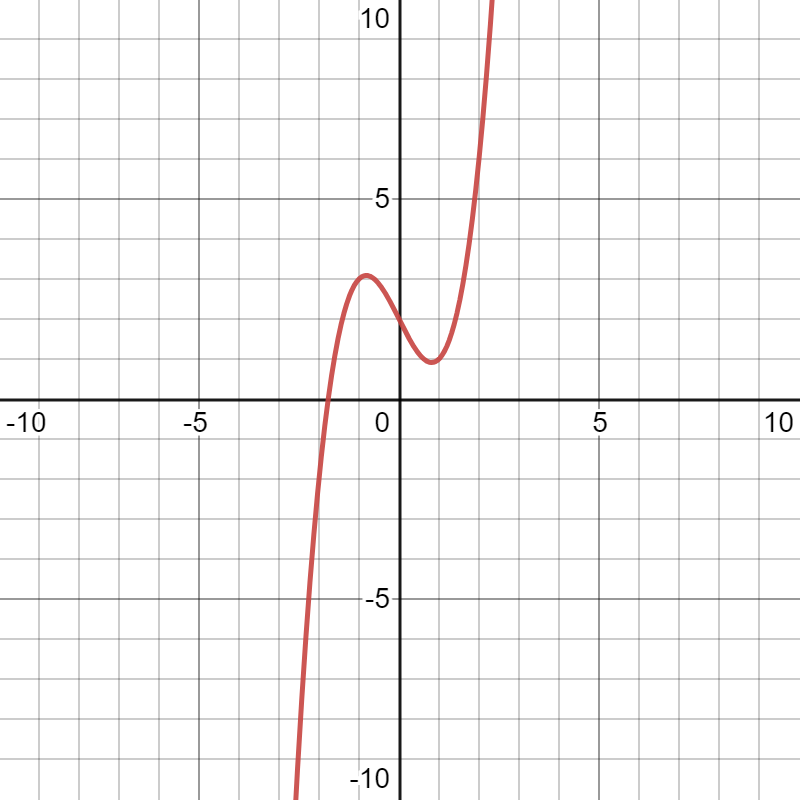
\includegraphics[width=10cm]{f3.png}
    \caption{$f_{3}(x)$}
    \label{fig:f3}
    \end{figure}

\begin{figure}[h]
    \centering
    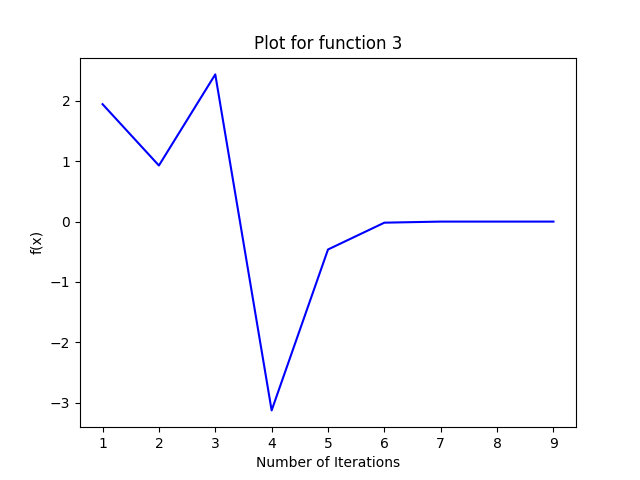
\includegraphics[width=10cm]{NME.png}
    \caption{$f_{3}(x) vs NMAX$}
    \label{fig:NME}
    \end{figure}
   
\begin{table}[]
\centering
\begin{tabular}{|c|l|l|l|}
\hline
\textbf{iter} & \multicolumn{1}{c|}{\textbf{xi}} & \multicolumn{1}{c|}{\textbf{correction}} & \multicolumn{1}{c|}{\textbf{rdiff}} \\ \hline
\textbf{1} & 1.400000000000  & 0.600000000000 & 0.300000000000 \\ \hline
\textbf{2} & 0.898969072165  & 0.501030927835 & 0.357879234168 \\ \hline
\textbf{3} & -1.288779327665 & 2.187748399830 & 2.433619206233 \\ \hline
\textbf{4} & -2.105767299014 & 0.816987971348 & 0.633923864086 \\ \hline
\textbf{5} & -1.829199950460 & 0.276567348553 & 0.131338039432 \\ \hline
\textbf{6} & -1.771715812062 & 0.057484138398 & 0.031425836407 \\ \hline
\textbf{7} & -1.769296561156 & 0.002419250906 & 0.001365484741 \\ \hline
\textbf{8} & -1.769292354251 & 0.000004206904 & 0.000002377727 \\ \hline
\textbf{9} & -1.769292354239 & 0.000000000013 & 0.000000000007 \\ \hline
\end{tabular}
\caption{Iteration Values for $f_{3}(x)$ obtained using \textbf{Newton's Method}}
\label{table:NME}
\end{table}
\chapter{Conclusion}
In conclusion, we have presented and discussed the theory, iteration method, python implementation and examples corresponding to Bisection, Newton and Secant Methods and also presented in an order way, the plots and tables corresponding to each Root Finding Algorithm.\\
In addition to that, we were asked to make a comment on the relative execution of the various Root Finding Algorithms. But that proved to be an incredible difficult task because of the philosophy being staggered and not continuous.In other words, what evaluation metrics should one adapt to make a statement? Number of iterations, CPU run-time and so on, are two of numerous metric parameters. But the most problematic factor is the way codes for different methods are written, as that itself can have a cascading effect when measuring relative execution speeds.\\
(Refer~\href{https://www.mdpi.com/2227-7390/9/11/1306/htm}{MPDI} for qualtitave and qualitative discussions)
For the detailed codes in Python, please visit \href{https://github.com/YashIITM/Root-Finding-Algorithms}{github}.

    \printbibliography

    \appendix

  
\end{document}
